\documentclass[a4paper, 12pt, addpoints]{exam}
\usepackage{IfbaProvas}
\newpage\backgroundsetup{contents={}} %Não imprimir plano de fundo (caso queira é só comentar a linha)
%==============================================================
\printanswers% para imprimir soluções
%\noprintanswers % Não imprimir soluções
%==============================================================
\tipoAvaliacao{1ª Avaliação Teórica}
%==============================================================
%=========================================================
%------------Cabeçalho e rodapé 
%=========================================================
\pagestyle{headandfoot}%{head}%empty
\firstpageheader{}{}{}
\runningheader{\disciplina}{}{\avaliacao}
\runningheadrule
\firstpagefooter{\professor}{}{Pag. \thepage\ de \numpages}
\runningfooter{\professor}{}{Pag. \thepage\ de \numpages}
\runningfootrule
%===============================================================
%INFORMAÇÕES SOBRE A AVALIAÇÃO
\nomeInst{Instituto Federal do Ceará}
\logoInst{
\includegraphics[scale=0.4]{Figs/ifbajequie.jpg}}
\Campus{Tauá} %COMENTE ESTA LINHA SE FOR ENSINO FUNDAMENTAL OU MÉDIO
\nomeCurso{Análise e Desenvolvimento de Sistemas} %Se não for curso superior, basta comentar esta linha
\nomeDisciplina{Ciência de Dados}
\DataProva{}
\Turma{}
\Semestre{5º}
\nomeProfessor{Prof. Reginaldo Fernandes}
\Aluno{}
\matriculaAluno{}
%Caso não queira imagem de fundo, basta comentar a linha abaixo
%\ImagemFundo{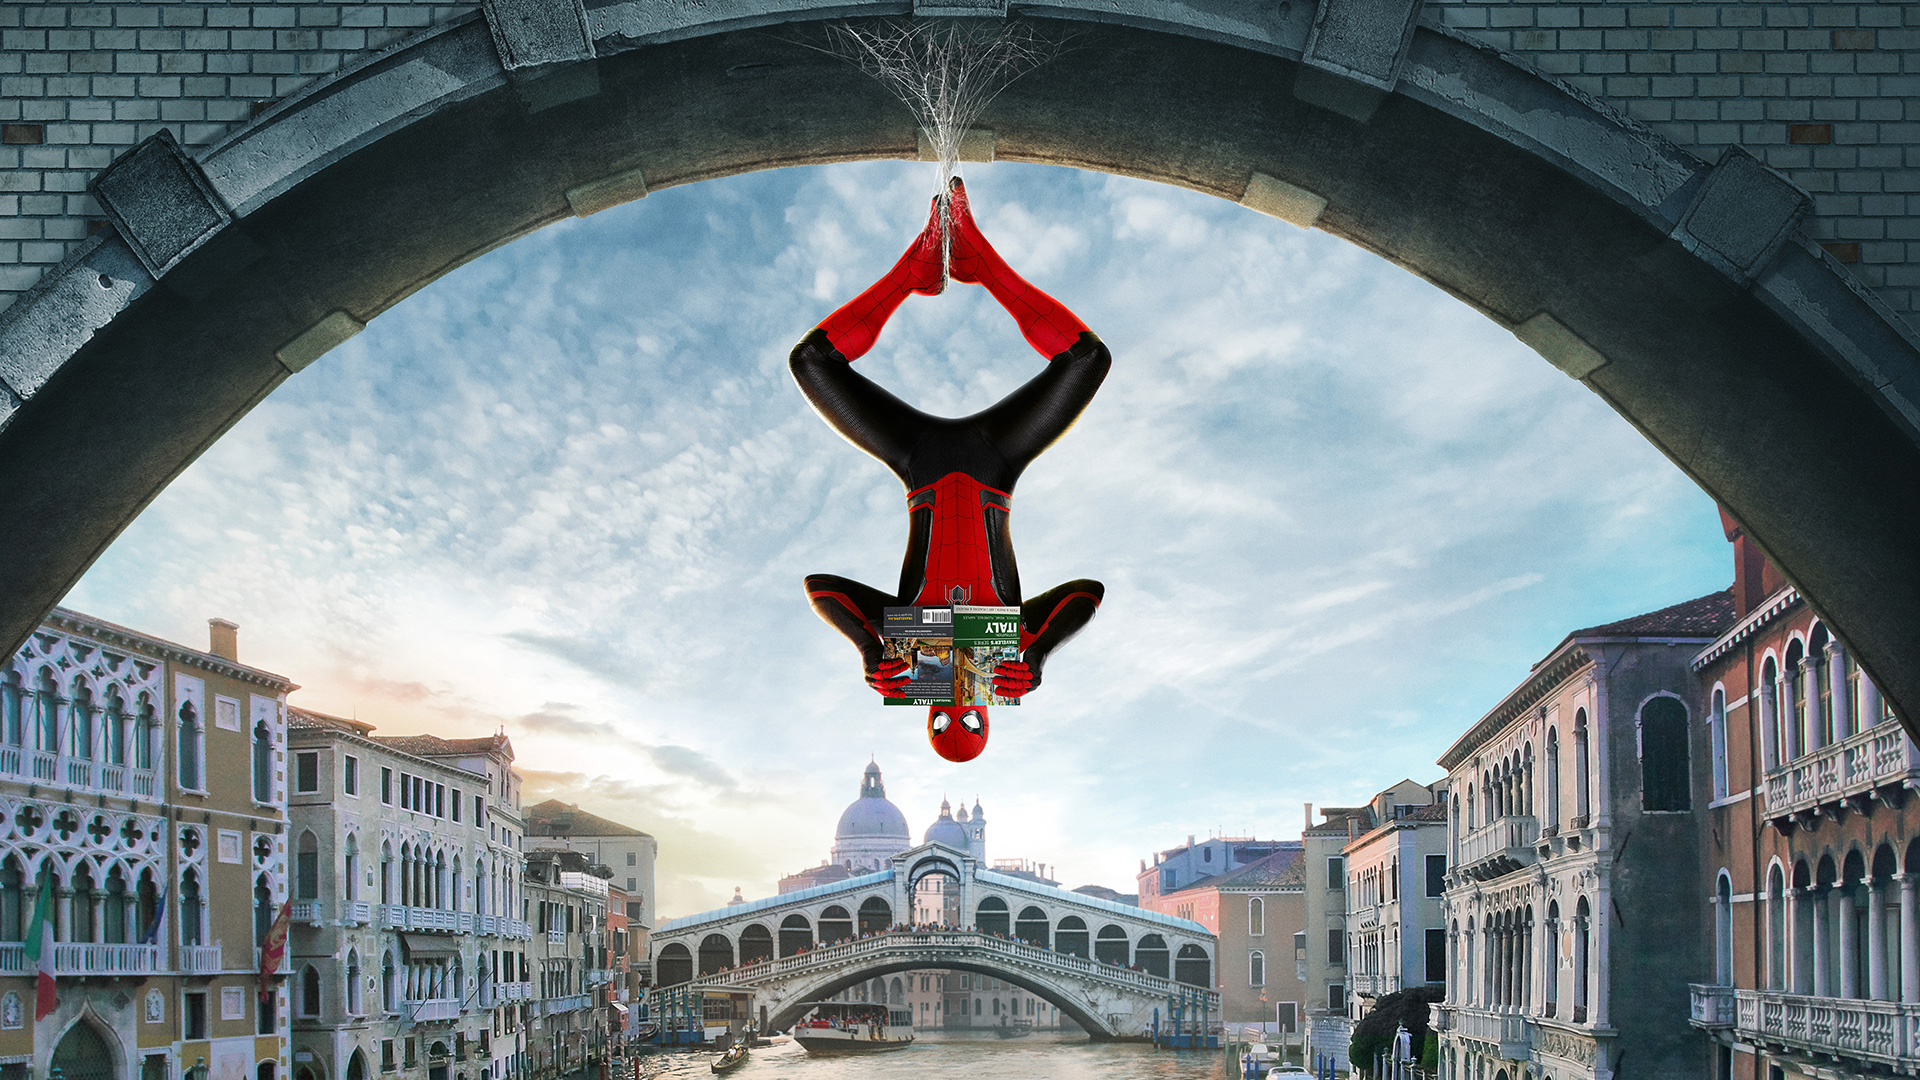
\includegraphics[height=\paperheight]{Figs/Fundo/aranha2.jpeg}}
%===============================================================

%INSTRUÇÕES PARA A AVALIAÇÃO, deixe em branco as que não quiser colocar
\instum{Sua avaliação consta de \numquestions \ questões, somando \numpoints \  pontos. \textbf{É proibido utilizar consultas.}} 
\instdois{\textbf{A posse de celular durante a avaliação será entendida como cola, independentemente do uso.}}
\insttres{}
\instquatro{}
\instcinco{}
\instseis{}
%==============================================================

%COMEÇO DO DOCUMENTO
\begin{document}
\info\vspace{-1.2 cm} %Imprime as informações do cabeçalho programada no pacote 
%TABELA DE PONTUAÇÃO E PESOS
\begin{center}
\scalebox{0.923}{
	\gradetable[h]
}
\end{center}

\begin{questions}
	
	\question[1]
	Um estudo observacional identificou que pessoas que consomem chocolate regularmente apresentam menor incidência de doenças cardiovasculares.
	
	Explique por que essa observação não é suficiente para concluir que o consumo de chocolate causa melhora da saúde cardiovascular. Cite duas possíveis variáveis de confusão e explique como elas podem afetar a interpretação dos resultados.
	
	\question[1]
	
	Explique o papel da randomização em um experimento controlado.
	
	Na sua resposta, descreva:
	
	\begin{parts}
		\part O que é um grupo de tratamento;
		\part O que é um grupo de controle;
		\part Como a randomização reduz o efeito das variáveis de confusão.
	\end{parts}
	
	\question[1]
	
	O conceito de \textit{ceteris paribus} é frequentemente utilizado em estudos observacionais.
	
	Explique:
	
	\begin{parts}
		\part O significado da expressão;
		\part Por que ela é importante na inferência causal;
		\part Por que é mais difícil obter um cenário \textit{ceteris paribus} em estudos observacionais do que em experimentos controlados.
	\end{parts}
	
	\question[1]
	
	Considere um estudo que deseja analisar o perfil dos estudantes universitários brasileiros.
	
	Foram coletadas respostas apenas de usuários ativos de uma rede social específica.
	
	Explique a diferença entre:
	
	\begin{parts}
		\part População-alvo;
		\part Estrutura de acesso (\textit{access frame});
		\part Amostra coletada.
	\end{parts}
	
	Discuta também como um viés de seleção pode comprometer os resultados do estudo mesmo quando milhões de respostas são obtidas.
	\vspace{1cm}
	\question[1]
	
	Defina os conceitos de:
	
	\begin{parts}
		\part Parâmetro populacional;
		\part Estimador;
		\part Estimativa.
	\end{parts}
	
	Explique por que a média amostral é considerada uma variável aleatória enquanto a média populacional é um valor fixo.
	
	
	
	
	\question[1]
	
	Considere uma moeda justa.
	
	Explique o que afirma a Lei dos Grandes Números e por que ela é importante para a construção de modelos estatísticos.
	
	Utilize o lançamento de moedas como exemplo.
	
	
	\question[1]
	
	Considere dois modelos de previsão:
	
	\begin{itemize}
		\item Modelo A: produz resultados muito próximos entre si, porém sistematicamente acima do valor real.
		\item Modelo B: produz resultados centrados no valor real, porém bastante dispersos.
	\end{itemize}
	
	Identifique qual modelo apresenta:
	
	\begin{parts}
		\part Alto viés e baixa variância;
		\part Baixo viés e alta variância.
	\end{parts}
	
	Explique os riscos de cada situação para aplicações de Ciência de Dados.
	
	\question[1]
	
	Classifique cada variável como \textbf{discreta} ou \textbf{contínua}.
	
	\begin{enumerate}
		\item Número de alunos matriculados em uma disciplina.
		\item Tempo de resposta de um servidor.
		\item Quantidade de acessos a um sistema.
		\item Altura dos estudantes.
		\item Número de erros encontrados em um software.
	\end{enumerate}
	
	Justifique suas respostas.
	
	
	\question[1]
	
	Dale e Krueger realizaram um estudo para investigar uma questão bastante discutida: estudantes que frequentam universidades mais prestigiadas realmente obtêm salários maiores por causa da instituição ou porque já eram alunos mais qualificados antes de ingressarem nela?
	
	Para responder a essa pergunta, os pesquisadores analisaram estudantes que haviam se candidatado às mesmas universidades. Em vez de comparar apenas alunos de instituições diferentes, eles compararam estudantes com perfis acadêmicos semelhantes, utilizando informações sobre quais universidades os haviam aceitado ou rejeitado. Dessa forma, buscaram criar grupos mais comparáveis e reduzir o efeito de fatores externos.
	
	Com base nesse estudo, explique:
	
	\begin{parts}
		\part Por que comparar simplesmente alunos de universidades diferentes pode produzir conclusões equivocadas;
		
		\part Como o pareamento por aceitações e rejeições ajuda a aproximar um cenário de ``\textit{todo o resto igual}'';
		
		\part Qual problema metodológico essa estratégia procura reduzir.
	\end{parts}
	
	\question[1]
	
	Uma pesquisa deseja estimar a média das notas dos estudantes de uma instituição.
	
	Explique:
	
	\begin{parts}
		\part Por que o tamanho da amostra influencia a qualidade da estimativa;
		\part Por que uma amostra grande nem sempre é representativa;
		\part O que caracteriza uma amostra representativa.
	\end{parts}
	
	\question[1]
	
	Um cientista de dados precisa apresentar os seguintes resultados para a diretoria:
	
	\begin{enumerate}
		\item Evolução mensal da taxa de evasão dos alunos ao longo de três anos.
		\item Distribuição dos estudantes por curso.
		\item Relação entre horas de estudo e nota final dos alunos.
	\end{enumerate}
	
	Para cada situação, indique qual visualização é mais adequada entre:
	
	\begin{itemize}
		\item Gráfico de linhas;
		\item Gráfico de barras;
		\item Gráfico de dispersão;
		\item Gráfico de pizza.
	\end{itemize}
	
	Justifique sua escolha explicando qual característica dos dados torna a visualização adequada.
	
	\question[1]
	
	Uma empresa apresentou o gráfico abaixo para demonstrar o crescimento das vendas entre 2023 e 2024.
	
	\begin{center}
		\begin{minipage}{0.20\textwidth}
			\centering
			\begin{tabular}{|c|c|}
				\hline
				Ano & Vendas \\
				\hline
				2023 & 980 \\
				2024 & 1000 \\
				\hline
			\end{tabular}
		\end{minipage}
		\hfill
		\begin{minipage}{0.74\textwidth}
			\centering
			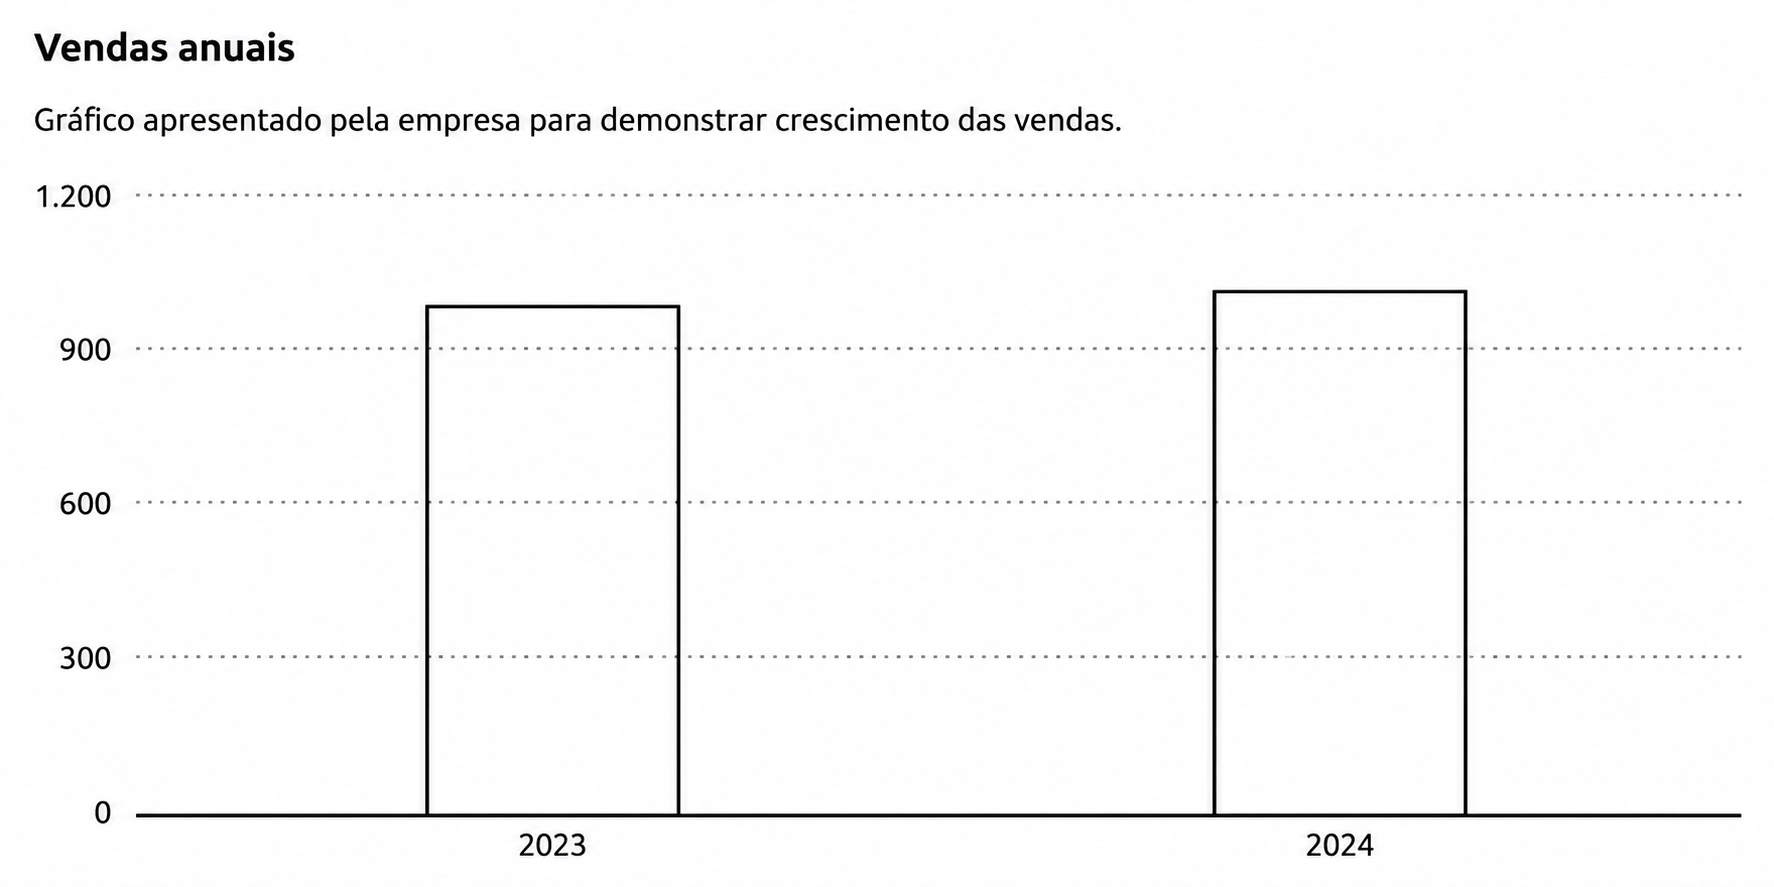
\includegraphics[width=\textwidth]{Figs/grafico_vendas.png}
		\end{minipage}
	\end{center}
	
	O analista informou que o eixo vertical do gráfico original foi configurado para iniciar em 950 e não em 0.
	
	Responda:
	
	\begin{parts}
		\part Por que iniciar o eixo vertical em 950 pode induzir interpretações equivocadas sobre os resultados?
		
		\part O crescimento apresentado parece maior ou menor do que realmente é? Justifique.
		
		\part Quais princípios de visualização de dados estão sendo violados nessa situação?
		
		\part Como o gráfico poderia ser redesenhado para representar os dados de forma mais transparente para os gestores?
		
		\part Calcule a variação percentual das vendas entre 2023 e 2024.
	\end{parts}
	
	
	\bonusquestion
	
	Escolha \textbf{apenas um} dos temas abaixo e desenvolva uma dissertação entre 10 e 20 linhas.
	
	\begin{enumerate}[A)]
		\item A importância da randomização para a inferência causal.
		
		\item Correlação não implica causalidade: explique o significado dessa afirmação e apresente um exemplo.
		
		\item O papel da amostragem na construção de conhecimento científico.
		
		\item Viés em Ciência de Dados: como ele surge e quais podem ser suas consequências.
		
		\item Como a visualização de dados pode influenciar a interpretação dos resultados de uma análise.
		
		\item Por que representatividade é tão importante quanto o tamanho da amostra.
	\end{enumerate}
	
	Sua resposta será avaliada pela clareza da argumentação, domínio conceitual e capacidade de relacionar os conceitos estudados na disciplina com situações práticas.	
\end{questions}
\end{document}